\documentclass[a4paper,oneside,12pt]{book}
%% === nezbytné balíčky:
\usepackage[T1]{fontenc}   % písmo pro UTF-8
\usepackage[utf8]{inputenc} % vstupní znaková sada UTF-8 || [cp1250] -> Windows 1250 || [latin2] -> ISO Latin 2

\usepackage{fvextra}  % nahrát před balíčkem csquotes!
\usepackage[autostyle]{csquotes}
%% citace zdrojů (BibLaTeX!):
\usepackage[style=iso-numeric]{biblatex} % očíslované citace typu "[1]". Jiná varianta: iso-authoryear vytiskne "(příjmení, rok)". BibLaTex: https://at.ctan.niranjan.co/macros/latex/contrib/biblatex-contrib/biblatex-iso690/biblatex-iso690.pdf + https://www.overleaf.com/learn/latex/Bibliography_management_with_biblatex
%\usepackage[authoryear]{natbib}
\addbibresource{literatura.bib} % zde lze změnit název .bib-souboru

\usepackage[czech]{babel} % česky psaná práce, typografická pravidla

\usepackage{pdfpages} % pokud nemáte formulář "Zadání bak./dipl. práce" naskenovaný jako PDF, tak ZAKOMENTUJTE

%\usepackage{encxvlna} % postará se o spojky a předložky, které dle českých pravidel nesmí být na konci řádku. Dokumentace: http://texdoc.net/texmf-dist/doc/generic/encxvlna/encxvlna.pdf

\usepackage[a4paper, hmarginratio=1:1]{geometry} % využití celé A4 stránky a nastavení okrajů, pro OBOUSTRANNÝ TISK

%% === balíčky, které se mohou hodit:
\usepackage[dvipsnames]{xcolor} % barvy
\usepackage{hyperref} % https://polish-mirror.evolution-host.com/ctan/macros/latex/contrib/hyperref/doc/hyperref-doc.pdf)
\hypersetup{ % nastavení pro balíček hyperref
    colorlinks = true, % barevné odkazy ("hidelinks" nic neobarví ani neorámuje)
    linkcolor = RedViolet, % odkazy uvnitř dokumentu (\ref, \pageref, \eqref)
    citecolor = RedViolet, % odkazy na citace
    urlcolor = RoyalBlue, % odkazy na URL
    filecolor = RoyalBlue, % odkazy na soubory
}
\usepackage{graphicx} % balíček pro vkládání RASTROVÝCH grafických souborů (PNG apod.)
%\usepackage{epsfig} % balíčky pro vkládání VEKTOROVÝCH grafických souborů typu EPS

%\usepackage{float} % rozšířené možnosti umístění obrázků
%\usepackage{caption} % pro popisky obrázků, tabulek atd.

\usepackage{booktabs} % https://ctan.org/pkg/booktabs
%\usepackage{tabularx} % jiný balíček pro rozšířené možnosti tabulek: https://ctan.org/pkg/tabularx
%\usepackage{tabu} % jiný balíček pro rozšířené možnosti tabulek: https://ctan.org/pkg/tabu
%\usepackage{longtable} % balíček pro tabulky přes více stránek

\usepackage{minted}  % balíček pro ukázky kódu
%\usepackage{listings}  % jiný balíček pro ukázky kódu

\usepackage{amsmath} % balíček pro pokročilou matematickou sazbu
%\usepackage{color} % pro možnost barevného textu
%\usepackage{fancybox} % umožňuje pokročilé rámečkování
%\usepackage{index} % nutno použít v případě tvorby rejstříku balíčkem makeindex
%\newindex{default}{idx}{ind}{Rejstřík} % zavádí rejstřík v případě použití balíku index


\topmargin=-15mm      % horní okraj trochu menší
\textwidth=150mm      % šířka textu na stránce
\textheight=240mm     % "výška" textu na stránce

\frenchspacing % za větou bude mezislovní mezera (v anglických textech je mezera za větou delší)
\widowpenalty=1000 % "síla" zákazu vdov (= jeden řádek odstavce na konci stránky)
\clubpenalty=1000 % "síla" zákazu sirotků (= jeden řádek/slovo odstavce samostatně na začátku stránky)
\brokenpenalty=1000 % "síla" zákazu zlomu stránky za řádkem, který má na konci rozdělené slovo

\pagenumbering{arabic} % číslování stránek arabskými číslicemi
\pagestyle{plain}      % stránky číslované dole uprostřed

\parindent=0pt % odsazení 1. řádku odstavce
\parskip=7pt   % mezera mezi odstavci

\newcommand{\ti}{\textit} % zkrácený příkaz pro kurzívu
\newcommand{\tb}{\textbf} % zkrácený příkaz pro tučné písmo


%% --- zde jsou makra, tj. "konstanty" - některé musíte změnit! --- %%
\newcommand{\cvut}{České vysoké učení technické v~Praze}
\newcommand{\fjfi}{Fakulta jaderná a fyzikálně inženýrská}
\newcommand{\katedra}{Katedra softwarového inženýrství}
\newcommand{\program}{Aplikace informatiky v~přírodních vědách} % změňte, pokud máte jiný stud. program
\newcommand{\spec}{--} % změňte, pokud studijní program má specializaci

\newcommand{\druh}{Bakalářská práce} % nebo "Diplomová práce"

\newcommand{\logoCVUT}{
\includegraphics{symbol_cvut_konturova_verze_cb.pdf}} % logo ČVUT -- podle grafického manuálu ČVUT platného od prosince 2016. Pokud nevyhovuje PDF-verze, tak použijte jinou variantu loga: https://www.cvut.cz/logo-a-graficky-manual -> "Symbol a logo ČVUT v Praze"). Pokud chcete logo úplně vynechat, zadejte místo "\includegraphics{...}" text "\vspace{35mm}"

% přesně podle formuláře "Zadání bak./dipl. práce" VYPLŇTE:
\newcommand{\nazevcz}{Český název práce}    % český název práce (přesně podle zadání!)
\newcommand{\nazeven}{Title in English}          % anglický název práce (přesně podle zadání!)
\newcommand{\autor}{Jméno Příjmení}   % vyplňte své jméno a příjmení (s akademickým titulem, máte-li jej)
\newcommand{\vedouci}{JménoV PříjmeníV} % vyplňte jméno a příjmení vedoucího práce, včetně titulů, např.: Doc. Ing. Ivo Malý, Ph.D.
\newcommand{\pracovisteVed}{\katedra, \fjfi, \cvut} % ZMĚŇTE, pokud vedoucí Vaší práce není z KSI
\newcommand{\konzultant}{--} % POKUD MÁTE určeného konzultanta, NAPIŠTE jeho jméno a příjmení + tituly
\newcommand{\pracovisteKonz}{--} % POKUD MÁTE konzultanta, NAPIŠTE jeho pracoviště

% podle skutečnosti VYPLŇTE:
\newcommand{\rok}{2023}  % rok odevzdání práce (jen rok odevzdání, nikoli celý akademický rok!)
\newcommand{\kde}{Praze} % studenti z Děčína ZMĚNÍ na: "Děčíně" (doplní se k "prohlášení")

\newcommand{\klicova}{Klíčová slova}   % zde NAPIŠTE česky cca 3-5 klíčových slov
\newcommand{\keyword}{Key words}       % zde NAPIŠTE anglicky cca 3-5 klíčových slov (přeložte z češtiny, ale odborně)
\newcommand{\abstrCZ}{Popis práce česky. Uveďte: téma a kontext práce, cíl práce, metodiku + použitá data, hlavní výsledky + co bylo dosaženo. Vše napište do~\textit{jednoho} odstavce, kde nejsou ani citace, ani odkazy do textu práce.}    % zde NAPIŠTE abstrakt v češtině (alespoň 7 vět, min. 80 slov. Pokuste se, aby CZ i EN abstrakt nezpůsobily přetečení strany 6 na stranu 7, tj. aby se obojí i s klíčovými slovy vešlo na JEDNU stránku. Obvykle mívá abstrakt 150-300 slov, to jest cca 5-12 řádků)
\newcommand{\abstrEN}{Popis práce anglicky} % zde NAPIŠTE abstrakt v angličtině


\newcommand{\podekovani}{Děkuji ... za ...} % NAPIŠTE (odborné) poděkování, např. svému vedoucímu:
% Děkuji Ing. Eleonoře Krtečkové, Ph.D. za vedení mé bakalářské práce a~za podnětné návrhy, které ji obohatily.
%--- nebo: ---
% Děkuji vedoucímu práce doc. Ing. Pafnutijovi Snědldítětikaši, Ph.D. za neocenitelné rady a~pomoc při tvorbě bakalářské práce.


\begin{document}
%%%%%%%%%%%% TITULNÍ STRANA -- následujících cca 30 řádků se generuje AUTOMATICKY. Neměňte!!! Výjimka: práce psané v angličtině! %%%%%%%%%%%%
\thispagestyle{empty}

\begin{center}
    {\Large \textsc{\cvut}\\[4mm] \textsc{\fjfi}}\par
    \vspace{4mm}
	\tb{\katedra} \par\vspace{3mm}

    \begin{tabular}{l}
		\tb{Studijní program: \program}\\
		\tb{Specializace: \spec}\\
    \end{tabular}

   \vspace{10mm} \logoCVUT \vspace{15mm}

   {\huge \tb{\nazevcz}\par}
   \vspace{5mm}
   {\huge \tb{\nazeven}\par}

   \vspace{15mm}
   {\Large \MakeUppercase{\druh}}

   \vfill
   {\large
    \begin{tabular}{ll}
    Vypracoval: & \autor\\
    Vedoucí práce: & \vedouci\\
    Rok: & \rok
    \end{tabular}
   }
\end{center}

%%%%%%%%%%%% ZADÁNÍ PRÁCE - z KOSu %%%%%%%%%%%%
% Zadání (podepsané děkanem atd.) si stáhnete v PDF z KOSu
\newpage  % SEM NESAHEJTE!
\thispagestyle{empty} % SEM NESAHEJTE!

%% ZADÁNÍ PRÁCE stažené z webKOS (nechte odkomentovanou jednu možnost!):
%\includepdf[pages={1}]{zadani_cele.pdf} % PDF má 1 stránku
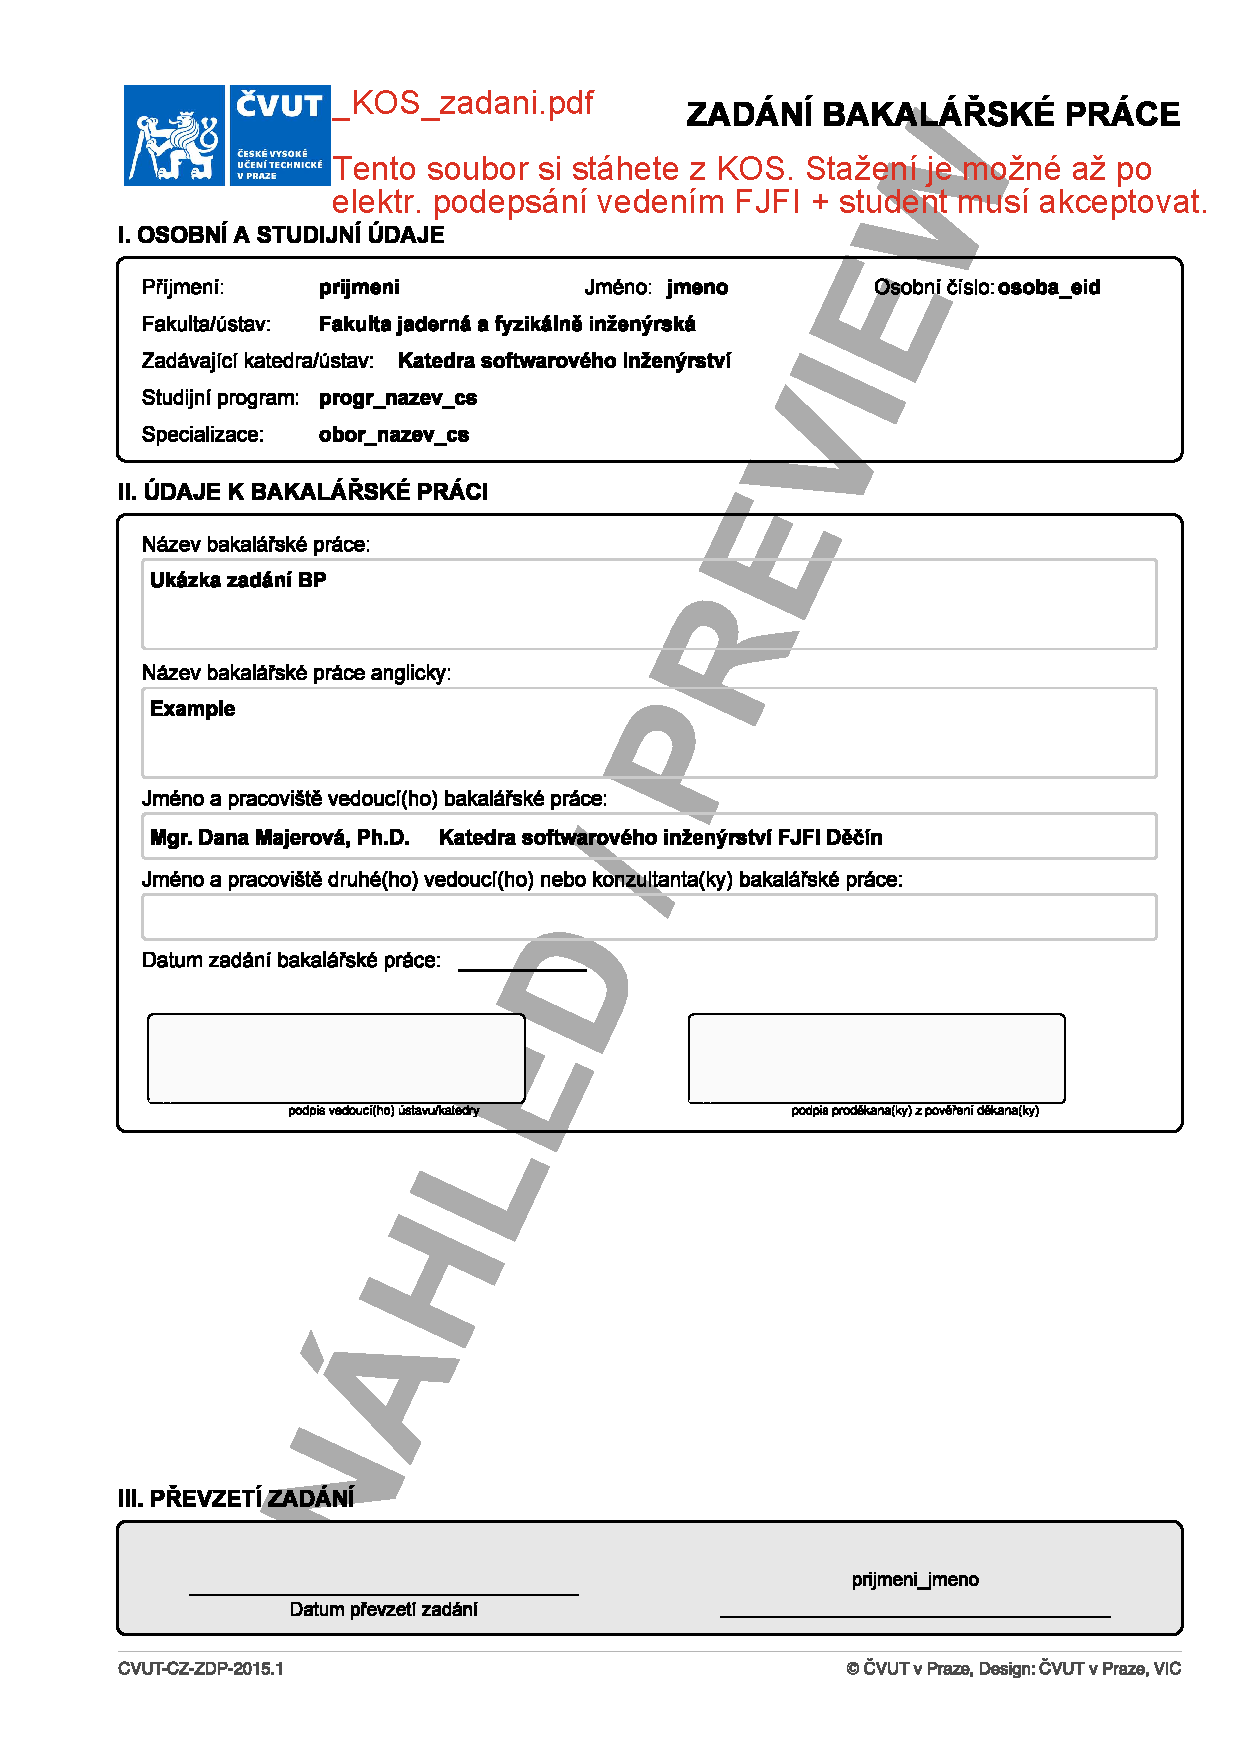
\includepdf[pages={1,2}]{_KOS_zadani.pdf} % PDF má 2 stránky
%% POZOR: pokud překladač (OverLeaf?) odstraní datum a elektr. podpisy, tak je potřeba ve výsledném PDF stránku/stránky VYMĚNIT ... s využitím nástrojů, které nevkládají vodotisk (např. webový  ilovepdf.com)


%%%%%%%%%%%% Prohlášení - z KOSu => vložte samostatné PDF %%%%%%%%%%%%
\newpage % SEM NESAHEJTE!
\thispagestyle{empty}  % SEM NESAHEJTE!

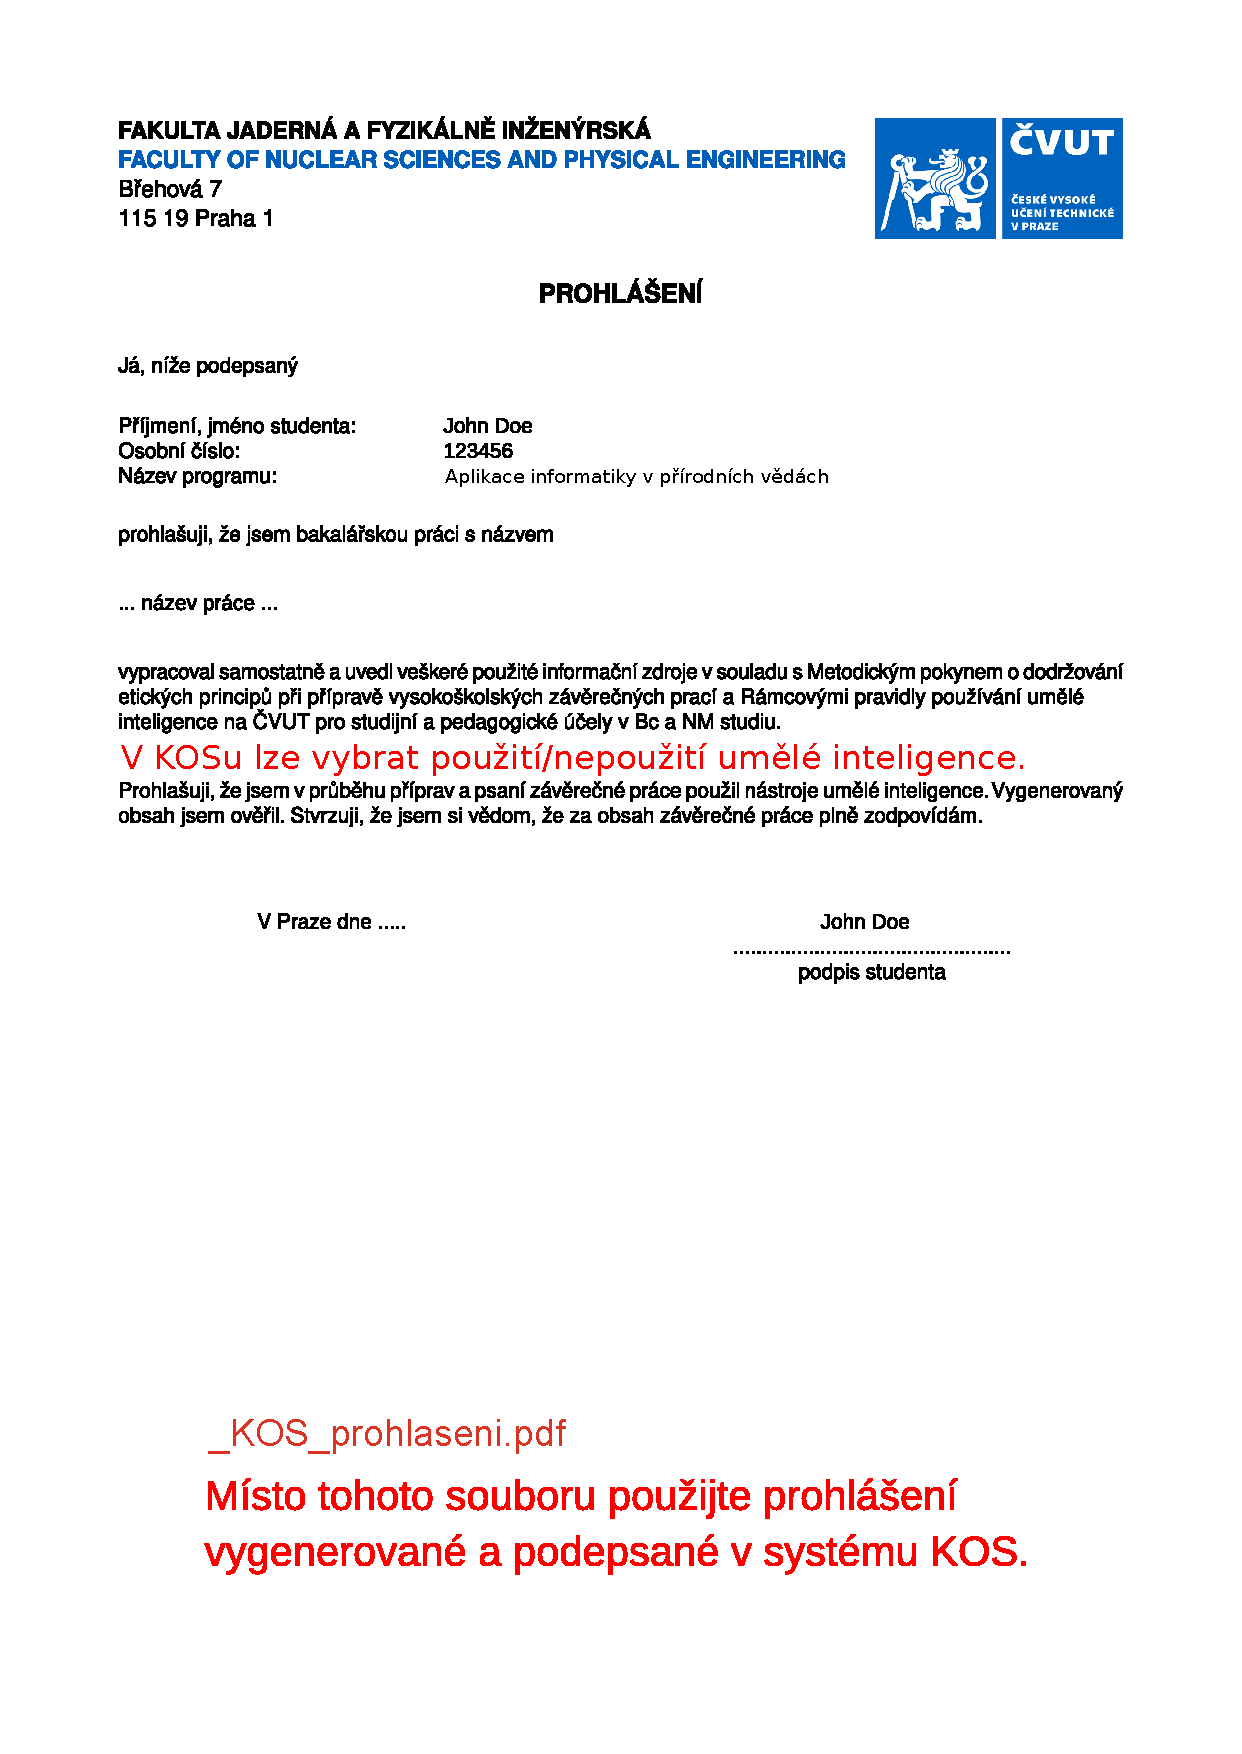
\includepdf[pages={1}]{_KOS_prohlaseni.pdf} % prohlášení o použití/nepoužití AI "podepíšete", a pak si stáhnete ve webKOS co nejpozději před odevzdáním (ideálně v den odevzdání)


%%%%%%%%%%%% Poděkování -- tuto stránku můžete celou odstranit %%%%%%%%%%%%
\newpage
\thispagestyle{empty}

~
\vfill % prázdné místo

\tb{Poděkování}

\vspace{1em} % vertikální mezera
\podekovani
\begin{flushright}
\autor
\end{flushright}  % <------- tady končí stránka s poděkováním


%%%%%%%%%%%% ABSTRAKT atp. Generuje se AUTOMATICKY podle maker nastavených na začátku souboru) %%%%%%%%%%%%
\newpage   % SEM NESAHEJTE!
\thispagestyle{empty}   % SEM NESAHEJTE!

% příprava:    (na následujících 8 řádků NESAHEJTE!)
\newbox\odstavecbox
\newlength\vyskaodstavce
\newcommand\odstavec[2]{%
    \setbox\odstavecbox=\hbox{%
         \parbox[t]{#1}{#2\vrule width 0pt depth 4pt}}%
    \global\vyskaodstavce=\dp\odstavecbox
    \box\odstavecbox}
\newcommand{\delka}{120mm} % šířka textů ve 2. sloupci tabulky

% použití přípravy:    % dovnitř "tabular" vůbec NESAHEJTE!
\begin{tabular}{ll}
  {\em Název práce:} & ~ \\
  \multicolumn{2}{l}{\odstavec{\textwidth}{\bf \nazevcz}} \\[1em]
  {\em Autor:} & \autor \\[1em]
  {\em Studijní program:} & \program \\
  {\em Specializace:} & \spec \\
  {\em Druh práce:} & \druh \\[1em]
  {\em Vedoucí práce:} & \odstavec{\delka}{\vedouci\\ \pracovisteVed} \\
  {\em Konzultant:} & -- %\odstavec{\delka}{\konzultant \\ \pracovisteKonz}  % VYMAŽTE text "-- %" v případě, že jste neměli konzultanta
 \\[1em]
  \multicolumn{2}{l}{\odstavec{\textwidth}{{\em Abstrakt:} ~ \abstrCZ  }} \\[1em]
  {\em Klíčová slova:} & \odstavec{\delka}{\klicova} \\[2em]

  {\em Title:} & ~\\
  \multicolumn{2}{l}{\odstavec{\textwidth}{\bf \nazeven}}\\[1em]
  {\em Author:} & \autor \\[1em]
  \multicolumn{2}{l}{\odstavec{\textwidth}{{\em Abstract:} ~ \abstrEN  }} \\[1em]
  {\em Key words:} & \odstavec{\delka}{\keyword}
\end{tabular}



%%%%%%%%%%%% Obsah práce ... je generován AUTOMATICKY %%%%%%%%%%%%
\newpage  % SEM NESAHEJTE!
\parskip=0pt
\tableofcontents % SEM NESAHEJTE!
\parskip=7pt
\newpage % SEM NESAHEJTE!


%--------------------------------------------------------
%|         Zde začíná SAMOTNÁ PRÁCE (text)              |
%--------------------------------------------------------

\chapter*{Úvod} % SEM NESAHEJTE!
\addcontentsline{toc}{chapter}{Úvod} % SEM NESAHEJTE!
%
Zde napište text úvodu (1-3 strany) nebo si text vložte ze samostatného souboru, např. příkazem \texttt{\textbackslash input\{vnitrek\_uvod.tex\}}.\par Text v~úvodu se nerozdělujte na podkapitoly, nýbrž na jednotlivé odstavce. Odstavce od sebe oddělíte prázdným řádkem nebo příkazem \texttt{\textbackslash par}. \par Úvod práce by měl obsahovat:
\begin{itemize}
    \item vymezení tématu práce (resp. problému), relevance tématu (význam/role řešeného problému v~celém ekosystému/prostoru problémů),
    \item motivaci (odborný důvod) výběru tématu,
    \item vymezení cíle/cílů práce (resp. smysl řešení daného problému),
    \item způsob/metodu dosažení cíle (stručný nástin řešení problému), výzkumné otázky či hypotézy,
    \item předpoklady či omezení práce.
\end{itemize}
Dále můžete čtenářům nastínit strukturu práce (tj. co v~které kapitole najdou). \par
Další informace čerpejte např. z~knih \cite{Kapounova2017} nebo \cite{Mesko2006}.
%
%\input{vnitrek_uvod.tex} % vložení souboru, který obsahuje text úvodu (bez nadpisu!)



\chapter{Jak psát závěrečnou práci} % změňte text kapitoly (pokud je \chapter součástí vkládaného souboru, tak tento řádek zakomentujte)
%
\small % zmenšení velikosti písma, aby pokyny byly kratší :-)
Tento text, vložený do \uv{šablony} příkazem \texttt{\textbackslash input\{vnitrek\_kapitola1.tex\}}, slouží jako stručné pokyny\footnote{Podrobnější informace o~psaní závěrečné práce získáte v~rámci předmětu \uv{Seminář k~bakalářské práci} (resp. \uv{Seminář k~diplomové práci}).} pro psaní závěrečné práce a~zároveň jej můžete využít jako ukázku práce v~\LaTeX{u}. Šablona pro psaní závěrečné práce je ke stažení na webu KSI~\cite{KSIweb2026}. Celý projekt byl přeložen pomocí Overleaf~\cite{overleaf2026}.
\par 
Ve skutečné závěrečné práci nahraďte soubor \texttt{vnitrek\_kapitola1.tex} za jiný (nebo kompletně přepište obsah souboru).

\newcommand{\prikaz}[1]{\texttt{\textbackslash #1\{\}}} % pomocné makro, definice by měla být spíše v preambuli, ale jelikož slouží pouze pro kapitolu~1 (a~ne pro všechny studenty), tak je umístěno zde

 
\section{Obsah textu} \label{obsah} 
Obsah závěrečné práce musí pokrýt všechny body z~osnovy (formulář \uv{Zadání bak./dipl. práce} lze stáhnout z~KOS, jakmile je zadání schváleno vedením FJFI a~akceptováno studentem). Rozšíření zadání práce není zakázáno, avšak vynechání některého bodu je považováno za nesplnění cílů práce.
\par 
Textová část práce musí být {\color{red} autorským dílem studenta} -- vyhýbejte se tedy jakýmkoliv pokusům o~plagiátorství. Použití nástrojů umělé inteligence deklarujete v~prohlášení (generováno v~KOS před odevzdáním práce $\Rightarrow$ soubor \texttt{\_KOS\_prohlaseni.tex} pak použijete s~touto \uv{šablonou}). \par
Metodické pokyny ČVUT\footnote{Stav ke dni 23.\,6.\,2026. Metodické pokyny mohou přibývat.} vztahující se k~závěrečným pracím:\label{metodPokyny}
\begin{itemize}
    \item \textit{Rámcová pravidla používání umělé inteligence na ČVUT pro studijní a pedagogické účely v Bc a NM studiu} (\url{https://www.cvut.cz/legislativa-tykajici-se-studia#umela-inteligence}),
    \item \textit{Dodržování etických principů při přípravě vysokoškolských závěrečných prací} (\url{https://www.cvut.cz/legislativa-tykajici-se-studia#eticke-principy}).
\end{itemize} Vyhněte se nejednoznačnostem a~nejasnostem v~textu -- jako autor své práce nesete za text plnou zodpovědnost.
\par
Použité zdroje (knihy, webové stránky, software apod.) by měly být \textit{řádně} citovány. Seznam použitých zdrojů se uvádí na konci práce (generujte jej ideálně pomocí BibLaTeX), jednotlivé zdroje se citují příkazem \prikaz{cite}. Podrobnosti naleznete v~sekci~\ref{podkapZdroje}.
\par
Teoretická část práce mívá nejméně 10~stran. Z~textu musí být jasně patrné, co je převzato z~literatury a~co jsou původní myšlenky studenta. Teorie by měla souviset s~výsledkem závěrečné práce.
\par 
Praktická část práce by měla popsat/obsahovat dosažené výsledky (např. funkční program, číselný výsledek řešení, nové pravdivé řešení dokázané v~rámci teorie, objektivně zdůvodněné rozhodnutí). Konkrétní výsledek je zvýrazněn v~závěru práce a~bez teorie uvedené v~práci ho není možné dosáhnout. Výsledky práce by měly přinášet nějaké nové informace a~vlastní pohled studenta na zpracovávané téma.
\par
Samotná práce by měla být dobře strukturovaná a její jednotlivé části by na sebe měly {\em dobře logicky navazovat}. Důraz by měl být kladen na věcnost, odbornou úroveň, dobrou čtivost a~(je-li to možné) aktuálnost textu. Velmi důležitá je {\em faktická přesnost a~úplnost} (zejména při použití již neaktuálních zdrojů).
\par
{\bf Tipy:} vyhněte se používání nevysvětlených zkratek. Nepoužívejte \uv{odbornou hantýrku}. Vyhněte se výrokům, které se dají různě interpretovat. Nepoužívejte příliš dlouhé věty. 



\section{Členění textu do kapitol a~sekcí}
Závěrečná práce obvykle obsahuje 5-6 kapitol (včetně úvodu a~závěru, tj. očíslované kapitoly jsou obvykle tři až čtyři). Kapitoly lze rozdělit na podkapitoly a~tyto dále na jednotlivé sekce:
\begin{itemize}
\item kapitola: {\texttt{\textbackslash chapter\{Název\}}},
\item podkapitola (v~kapitole): {\texttt{\textbackslash section\{Název\}}},
\item sekce (v~podkapitole):  {\texttt{\textbackslash subsection\{Název\}}}.
\end{itemize}
{\color{red}Dělení do nižších úrovní se nepoužívá}, protože závěrečné práce nemají tak velký rozsah. 
\par
Velikost písmen v~názvech (pod)kapitol a~sekcí:
\begin{itemize}
    \item práce psaná v~češtině: u~prvního slova je  první písmeno velké, ostatní slova píšeme pouze malými písmeny, kromě vlastních jmen\footnote{Psaní velkých písmen: \url{https://prirucka.ujc.cas.cz/\#div180}.} (např. \uv{Trh v~České republice}, \uv{Velká Fermatova věta}, \uv{Detektory v~experimentu AMBER}),
    \item práce psaná v~angličtině: nadpisy se podobají anglickému názvu práce (vizte \url{https://ksi.fjfi.cvut.cz/bakalarske-studium/bp}, sekce \textit{Anglický název práce -- pravidla pro psaní velkých/malých písmen}).
\end{itemize}
\par 
{\bf Tipy:} 
\begin{enumerate}
\item Pokud nevíte, jak vhodně rozčlenit svůj text, {\em požádejte o~radu vedoucího\/} své práce (při pravidelných konzultacích).
\item Zdá se, že v~závěrečné práci potřebujete čtvrtou úroveň členění? Zvažte, zda z~nějaké podkapitoly neudělat novou kapitolu.
\item Je vhodné uložit si texty jednotlivých kapitol (nebo i~podkapitol) do samostatných souborů. Lépe/jednodušeji pak přeskupíte vybrané části, když zjistíte, že původní členění práce nebylo vhodné. \par Typickým znakem nevhodně členěné práce jsou \uv{malé} (cca čtyřstránkové) kapitoly a~mezi nimi jedna \uv{velká} 20stránková kapitola.
\item Definujte si v~preambuli \uv{šablony} \textit{vlastní makra} a~využívejte je pro sémantické odlišení pojmů: např. makro pro názvy tříd, makro pro názvy metod apod. Pokud v~textu později budete potřebovat změnit vzhled (např. názvy tříd tučným řezem písma), tak bude stačit pouhá změna uvnitř makra.\par 
Ukázka:\\
\texttt{\textbackslash newcommand\{\textbackslash trida\}[1]\{\textbackslash textt\{\#1\}\}} $\rightarrow$ definice makra v~preambuli\\
\texttt{Třída \textbackslash trida\{ŽÁK\} je odvozena od třídy \textbackslash trida\{OSOBA\}.} $\rightarrow$ použití v~textu
\item Pro psaní poznámek, které nemají být součástí finálního textu, si můžete přidat do \uv{šablony} balíček \texttt{todonotes} (\url{https://latex-tutorial.com/wp-content/uploads/2021/07/todonotes.pdf}).

\end{enumerate}

\section{Obrázky a tabulky}\label{sekceObrTab}

Text závěrečné práce je vhodné doplnit tabulkami nebo obrázky (grafy, diagramy užití apod.), abyste lépe ilustrovali své myšlenky nebo dosažené výsledky. 
\par 
Obrázky a~tabulky se vkládají do plovoucího prostředí (\texttt{figure}, \texttt{table}). {\color{red} Plovoucí prostředí si LaTeX umístí sám} (na typograficky vhodné místo -- typicky nahoru či naopak dolů na stránku. Občas se obrázky dostanou až na konec kapitoly, ale nejedná se o~chybu).
\par 
Popis obrázku/tabulky se píše do příkazu \prikaz{caption} a~měl by být stručný a {\em výstižný}. Obrázky mají popis dole, kdežto tabulky mají popis nahoře. Pokud je obrázek (resp. tabulka) převzatý, nezapomeňte na konci popisku citovat zdroj!
\par 
Do textu vždy {\em napište důvod použití\/} obrázku/tabulky a~{\color{red}odkažte se na něj/ni}:
\begin{itemize}
\item vytvoření odkazu: příkaz \prikaz{label} následovaný po příkazu \prikaz{caption},
\item sazba čísla odpovídajícího odkazu (tj. např. číslo obrázku): příkaz \prikaz{ref},
\item sazba čísla stránky, kde je odkaz: příkaz \prikaz{pageref}.
\end{itemize}   
Tabulky a~obrázky v~plovoucím prostředí používají své vlastní, {\em nezávislé číselné řady}. Z~toho vyplývá, že v~odkazech uvnitř textu musíme kromě čísla udat i~informaci o~tom, zda se jedná o~obrázek, anebo tabulku! Příklad: \texttt{vizte \underline{obrázek}\textasciitilde\textbackslash ref\{odkazObrA\}}.
\par

\subsection{Obrázky}
Obrázky se vkládají do plovoucího prostředí \texttt{figure}. Nesnažte se přesvědčit \LaTeX, aby byl obrázek umístěný uprostřed stránky! Porušilo by to typografická pravidla sazby.\par 
Formát obrázku volte pokud možno vektorový (tj. EPS nebo PS), protože se dají zvětšovat i~zmenšovat bez újmy na čitelnosti. Pokud máte k~dispozici obrázek pouze v~rastrovém formátu (např. PNG nebo schéma v~JPG), nakreslete jej znovu v~některém vektorovém grafickém programu nebo jej alespoň vygenerujte v~co nejlepším rozlišení. Nemá smysl konvertovat bitmapové obrázky do formátu EPS.
\par
\textbf{Ukázka:} níže jsou uvedeny příkazy pro vložení obrázku \texttt{graf.png}, na který se bude odkazovat pomocí návěští \textit{grafA}.
{\small
\begin{verbatim}
\begin{figure}
  \centering  % vycentrovat
  \includegraphics[scale=0.8]{graf.png} % soubor + měřítko 80 % (scale)
  \caption{Graf závislosti $y$ na $x$.} % popis obrázku
  \label{grafA} % návěští = definice odkazu na obrázek pro \ref{}
\end{figure}
\end{verbatim}
} % small
\par 
{\bf Tip:} pomocí balíčku TikZ (\url{https://texample.net/}) lze kreslit některé typy obrázků přímo v~textu práce. (Balíček TikZ přidáte příkazem \prikaz{usepackage} v~preambuli této \uv{šablony}.)

\subsection{Tabulky} 
Tabulky se vkládají do plovoucího prostředí \texttt{table}. Platí totéž co v případě obrázků:  umístění tabulky ponechte na {\LaTeX}u. Na tabulku se pak v~textu odkážete pomocí \prikaz{ref} (či \prikaz{pageref}). 
Pro sazbu tabulky\footnote{Pokud v~(diplomové) práci potřebujete uvést tabulky, které zabírají několik stran, tak využijte balíček {\tt longtable} (\url{https://ctan.org/pkg/longtable}). Dlouhé tabulky se umisťují do \textit{přílohy} práce (tj. jako \prikaz{chapter} za příkazem \texttt{\textbackslash appendix}).} lze využít např. balíček {\tt booktabs} $\Rightarrow$ profesionální tabulky s~proměnlivou tloušťkou čar (dokumentace: \url{https://ctan.org/pkg/booktabs}, ukázky: \url{https://people.inf.ethz.ch/markusp/teaching/guides/guide-tables.pdf}). \par
\textbf{Ukázka:} v~této \uv{šabloně} je tabulka~\ref{tabMakra} na str.~\pageref{tabMakra}, kde je přehled maker pro vygenerování úvodních stran práce (zdrojový kód tabulky: konec souboru \texttt{vnitrek\_kapitola1.tex}).

\textbf{Tip:} pokuste se dodržet \textit{stejné formátování tabulek} napříč celým textem práce (tj. aby v~jedné kapitole nebyly tabulky vzhledově odlišné od jiných kapitol).


\section{Pravidla českého pravopisu}\label{sekcePravidla}
Text česky psané práce by měl dodržovat pravidla českého pravopisu. Jako pomocník může posloužit např. \url{https://prirucka.ujc.cas.cz/}, kde nahoru do formuláře napíšete slovo a necháte si jej vyhledat (zda vůbec takové slovo existuje a~jak se skloňuje/časuje, resp. jak se používá).
\par 
{\bf Tip:} zapněte si v~Overleaf (resp. nainstalujte si do editoru pro \LaTeX) kontrolu českého pravopisu. Pokud si nejste čímkoli jisti, kupte/půjčte si aktuální \uv{Pravidla českého pravopisu} nebo požádejte o~kontrolu gramatických chyb osobu s~vytříbeným smyslem pro český jazyk (která se nebude zaměřovat na obsah práce, ale právě na stylistiku a pravopis). Pamatujte: není úkolem vedoucího práce, aby opravoval (a~četl) vaše pravopisné chyby!




\section{Typografická pravidla}\label{podkapTypo}
Text práce musí vyhovovat typografickým pravidlům. Pokud netušíte, o~co jde, vyhledejte si např. heslo \uv{Základní pravidla hladké sazby}.
\par 
Především se zaměřte na:
\begin{itemize}\itemsep=2pt
\item \textbf{pevná mezera} (znak {\tt \textasciitilde}) se píše mezi zkratkou jména a příjmením nebo mezi jednopísmennou předložkou/spojkou a~následujícím slovem. Mezi číslem a~jednotkou se píše {\bf úzká mezera} (znaky \texttt{\textbackslash,}). Ukázky: {\tt Bylo naměřeno 12,7\textbackslash,W.} nebo {\tt Dne 7.\textbackslash,1.\textbackslash,1610 objevil G.\textbackslash,Galilei 4\textasciitilde měsíce Jupiteru} apod.;
\item {\bf členicí (interpunkční) znaménka} $\rightarrow$ podrobnosti pod heslem \uv{Pravopis -- interpunkce} na webu \url{https://prirucka.ujc.cas.cz/}.\par
Základní typografická pravidla pro znaménka:\\
Tečka, čárka, středník, dvojtečka, otazník a vykřičník se přimykají k~předcházejícímu slovu bez mezery (mezera se píše až za nimi). Výjimkou je desetinná čárka (v~anglicky psané práci desetinná tečka), okolo které se mezery nepíšou;
\item {\bf pomlčka}\footnote{Pomlčka v~anglicky psané práci se sází jako \texttt{-{}-{}-} a bez mezer okolo.} a~{\bf spojovník} (spojovací čárka) jsou různé znaky! Pro spojovací čárku píšeme znak \texttt{-}, kdežto pomlčku sázíme jako \texttt{-{}-}.\par 
Kdy (a~jak) se používá pomlčka: \url{https://prirucka.ujc.cas.cz/?id=165}.\par 
Kdy se používá spojovník: \url{https://prirucka.ujc.cas.cz/?id=164};
\item {\bf závorky} se přimykají k~vnitřnímu textu, tedy mezera se píše před levou závorkou, a~pak za pravou závorkou;
\item \textbf{uvozovky} se přimykají k~vnitřnímu textu. V~česky psané práci můžete využít makro {\tt \textbackslash uv\{text\}}. 
\par
Pozor: pokud uvádíte ukázky zdrojového kódu programů, tak v~nich se používají uvozovky anglické (a také jiný typ písma).
\par Podrobnosti k~používání uvozovek: \url{https://prirucka.ujc.cas.cz/?id=162};
\item \textbf{apostrof} (odsuvník): \url{https://prirucka.ujc.cas.cz/?id=168};
\item \textbf{lomítko} jako oddělovač se píše bez mezer. Příklad: {\tt školní rok 2000/2001}; %
\item \textbf{procento} se sází se zpětným lomítkem. Pozor na rozdíly mezi 20\,\% (dvacet procent) a 20\% (dvacetiprocentní)! Podrobnosti: \url{https://prirucka.ujc.cas.cz/?id=790}.
\end{itemize}


\subsubsection*{Složení čísel a slov}
Jak správně psát slova složená z~čísel a~slov? Podrobnosti naleznete na: \url{https://prirucka.ujc.cas.cz/?id=790}.\par
Ukázka správného zápisu \uv{složenin} (všimněte si, že je to bez mezer a~bez spojovníku):\\
-- {\tt 20leté pozorování} nebo\\
-- {\tt dvacetileté pozorování}\\
(jakékoli jiné tvary jsou chybné!).
\par\vspace{-3mm}
\begin{tabbing}
Pozor na \textit{význam}: \ \= {\tt 5\,°} (s~úzkou mezerou) znamená \uv{pět stupňů},\\ \> {\tt 5°} (bez mezery) znamená \uv{pětistupňový}.
\end{tabbing}


\subsubsection*{Zvýrazňování textu}
Pro zvýraznění pojmů uvnitř textu se používá \textit{kurzíva} (příkaz \prikaz{textit} nebo lze využít \prikaz{ti} definované v~\uv{šabloně}).\par 
Silné zvýraznění (tj. tučné písmo) se v~závěrečných pracích uvnitř odstavců nepoužívá (nicméně existuje příkaz \prikaz{textbf} nebo  \prikaz{tb} ze \uv{šablony}).


\subsubsection*{Psaní výčtů}
Pro psaní výčtů lze v~\LaTeX{u} využít prostředí {\tt enumerate} (číslovaný seznam) nebo {\tt itemize} (odrážky), položky píšeme do {\tt \textbackslash item}. Pravidla: \url{https://prirucka.ujc.cas.cz/?id=870}.


\subsubsection*{Psaní zkratek}
O~psaní zkratek pojednává heslo \textit{Zkratky, značky, čísla a~číslovky} na webovém rozcestníku \url{https://prirucka.ujc.cas.cz/}.
Používáte-li ve své práci větší množství zkratek, vytvořte \textbf{seznam použitých zkratek} (umisťuje se mezi obsah a~úvod, řadí se abecedně).


\subsubsection*{Psaní značek}
Psaní značek, především matematických: \url{https://prirucka.ujc.cas.cz/?id=785}.

\subsubsection{Zalomení řádku nebo stránky}
\textbf{Zalomení řádku} (tj. vynucené ukončení řádku uvnitř odstavce) se používá v případech, kdy uvnitř odstavce přetéká text přes pravý okraj (a~nelze jej vhodně přeformulovat, aby se tím přetečení opravilo). Správný příkaz pro zalomení řádku je \texttt{\textbackslash linebreak} (\LaTeX\ pak správně prodlouží mezislovní mezery). Rozhodně nepoužívejte sekvenci \texttt{\textbackslash\textbackslash}, která porušuje plynulý tok textu v~odstavci.

\textbf{Zalomení stránky} (neboli \uv{tvrdý konec} stránky vynucený příkazem \texttt{\textbackslash newpage}) se vůbec nepoužívá. Nesnažte se pomocí něj o~\uv{přesné} rozmístění obrázků nebo tabulek!

\section{Sazba matematického textu}

Mezi nejdůležitější typografické zásady psaní matematického textu patří:
\begin{itemize}\itemsep=1pt
\item známé konstanty a čísla určitá se píšou vzpřímeným řezem (např. $124$, $\mathrm e$, $\mathrm{\pi}$, $1-3\mathrm i$),
\item obecné konstanty a proměnné se píšou kurzívou (např. $a$, $x$, $x_1$),
\item identifikátory vektorů a matic se sázejí tučným řezem písma, např. $\mathbf{v}$, $\mathbf{M}$,
\item názvy funkcí (resp. známých polynomů) se píšou vzpřímeným řezem (např. $\sin(x)$, $\exp(y)$, $\mathrm{p}(x)$),
\item diferenciály se píšou vzpřímeným řezem, příslušná proměnná pak kurzívou: $\mathrm{d}x$.
\end{itemize}

Příkazy pro matematickou sazbu jsou popsány též v~knize \textit{\LaTeX pro začátečníky} \cite{Rybicka2003}.


\subsection{Desetinné číslo v~matematickém režimu} \label{des_cislo}
V českém textu používáme u~čísel desetinnou {\em čárku}, avšak čárka je v~mate\-ma\-tickém režimu
chápána jako oddělovač prvků seznamu ($\Rightarrow$ \LaTeX\ za ni automaticky přidává mezeru), proto je nutno desetinnou čárku uzavírat do složených závorek: \\
zdrojový kód \dots\ {\tt \$a=21\{,\}7\$\textbackslash,cm}\\ 
výsledek \dots\ $a=21{,}7$\,cm.


\subsection{Odkazy na rovnice nebo vztahy}
Rovnice, na které se budete v~textu odvolávat, opatřete pořadovými čísly při pravém okraji příslušného řádku (např. prostředí {\tt equation}) a přidejte návěští (\prikaz{label}). Ukázka:
\begin{equation}\label{vzorec1}
p = \frac{1}{n}\cdot\sum_{i=1}^n c_i
\end{equation}

Číslování rovnic může být průběžné v~textu, nebo v~jednotlivých kapitolách, {\em odkaz na vzorec\/} vysází příkaz {\tt $\backslash$eqref\{odkaz\}} z~balíku {\tt amstex}, resp. napište \prikaz{ref} do závorek: {\tt ($\backslash$ref\{odkaz\})}.
%Příklad: \hspace*{10mm} Průměrnou hodnotu z~čísel $c_1,c_2,\ldots,c_n$ vypočteme podle vztahu \eqref{vzorec1}.



\section{Ukázky zdrojových kódů}
Pokud chcete v~textu své práce upozornit na nějaký \textit{obzvláště zajímavý} zdrojový kód, můžete zařadit krátkou ukázku (obvyklejší však je, že ukázky zdrojového kódu uvedete až do textové přílohy práce s~patřičným komentářem. Nebo je neuvádíte do textu vůbec a~ponecháte na čtenáři, zda se podívá do samostatné přílohy\footnote{O~přílohách-souborech pojednává sekce~\ref{nahraniPriloh}.} se zdrojovými kódy).

Prostředí pro sazbu zdrojových kódů:
\begin{itemize}
    \item prostředí {\tt minted} (balíček {\tt minted}) vypadá dle zkušeností nejlépe (a na Overleaf bez problému funguje).
    Dokumentace: \url{https://www.overleaf.com/learn/latex/Code_Highlighting_with_minted};
    \item prostředí {\tt lstlisting} (balíček {\tt listings}) lze přizpůsobit pomocí příkazu \prikaz{lstset}. Dokumentace: \url{https://ftp.mpi-inf.mpg.de/pub/tex/mirror/ftp.dante.de/pub/tex/macros/latex/contrib/listings/listings.pdf};
    \item prostředí {\tt verbatim} (bez balíčku) je spíše nouzová záležitost -- sází pouze černý text neproporcionálním písmem.
\end{itemize}





\section{Citace a formát seznamu použitých zdrojů}\label{podkapZdroje}

% Stručně: https://prirucka.ujc.cas.cz/?id=883
Česky psaná práce: pro práci s~bibliografickými citacemi se používá  česká technická norma ČSN~ISO~690 (ideálně poslední vydání\footnote{V~červnu\,2026 to byla norma ČSN~ISO~690:2022.}; manažer \textit{CitacePro} ji podporuje). Další informace: \url{https://knihovna.cvut.cz/seminare-a-vyuka/jak-psat/jak-citovat}.
\par
Ve své závěrečné práci využijete různé zdroje informací (je doporučeno pracovat s~knihami nebo články z~časopisů Q1/Q2, nikoli s~nerecenzovanými weby nebo s~informacemi halucinujících chatbotů). Text práce tedy bude obsahovat údaje, které nejsou původní, a~proto je potřeba zdůraznit, co není studentův text:
\begin{itemize}
\item citují se použité {\em zdroje, které se týkají obsahu práce} (nikoli zdroje související s~úpravou/formou závěrečné práce, jako např. příručka k~\LaTeX u),
\item citován by měl být vždy {\em originální zdroj} (nikoli stránka z~Wikpedie!). \par Pozn.: pokud se jedná o~nějaký všeobecně známý fakt, normu, resp. standard de~facto či de iure, tak není potřeba hledat zdroj (vizte \textit{Metodické pokyny ČVUT} zmíněné v~sekci~\ref{obsah} na straně~\pageref{metodPokyny}),
\item seznam použitých zdrojů je umístěn za závěrem práce,
\item citační styl pro ČSN ISO~690 v~BibLaTeXu: \texttt{iso-numeric} (řazení dle pořadí použití zdroje v~textu práce) nebo \texttt{iso-authoryear} (tzv. hardvardská metoda; seznam zdrojů se řadí abecedně). % abecedně dle příjmení autora. Pokud autor chybí, tak podle prvního slova. 

%Případně změňte podle doporučení školitele nebo podle zvyků v~daném oboru.
\end{itemize}

Dbejte na {\color{red}úplnost citace} $\Rightarrow$ uvádějte co nejvíce informací o~citovaném zdroji (např. číslo vydání dané knihy, název sborníku, číslo stránky ve sborníku, platný odkaz na článek). Jednoznačným identifikátorem by mělo být ISBN u~knih, ISSN u~časopisů nebo DOI u~elektronických článků.
\par 
Cituje se vše, co není původním textem autora. Technicky: jednotlivé zdroje se v~textu citují příkazem \texttt{\textbackslash cite\{id\}} nebo \texttt{\textbackslash cite[strana]\{id\}}, přičemž \texttt{id} je definováno jako návěští v~souboru \texttt{literatura.bib} (blíže v~sekci~\ref{kap-odkazy}). V~případě citace slova (resp. části věty) se citace uvádí hned za citovanou část (za mezeru), jinak se udává za větu, resp. za konec odstavce (za tečkou, s~mezerou). Pozn.: převzaté vzorce (resp. rovnice) je vhodné citovat každý zvlášť + s~číslem stránky dané knihy, aby si např. čtenář (typicky oponent práce) mohl dohledat jejich správnost.
\par 
\textbf{Tip:} pro správu citací můžete využít desktopovou aplikaci \textit{JabRef} (\url{https://www.jabref.org/}). Dále existuje webový citační manažer \textit{CitacePro} (\url{https://www.citacepro.com/}), kam lze citace průběžně ukládat (po přihlášení se \uv{pod hlavičkou ČVUT}), a~pak si uložené zdroje vyexportovat do \href{https://www.overleaf.com/learn/latex/Bibliography_management_with_biblatex}{BibLaTeX}u\footnote{Nemáte-li BibLaTeX, tak nouzově exportujte do TeX a~vhodně seřaďte, aby to odpovídalo ČSN ISO 690. V~\uv{šabloně} pak použijte variantu~B pro seznam použitých zdrojů.} $\Rightarrow$ vzniklý soubor přejmenujete na \texttt{literatura.bib}.
Pozor: záznamy hledané na \textit{CitacePro} např. podle ISBN \textit{nemusejí obsahovat relevantní informace} o~použitém zdroji $\Rightarrow$ vždy si nalezenou citaci \textit{zkontrolujte} podle originální knihy!



\section{Křížové odkazy} \label{kap-odkazy}
Pro odkazy na stránky, na čísla kapitol a podkapitol, na čísla obrázků a tabulek atd. využíváme
speciálních prostředků DTP programu, které zajistí vygenerování správného čísla i~v případě, že se
text posune díky změnám samotného textu nebo díky úpravě parametrů sazby. V~systému \LaTeX\ jde o~odkaz na číslo, které odpovídá umístění značky v~textu (tzv.~navěští).

\subsubsection{Definice návěští}

Návěští se definuje pomocí {\tt \textbackslash label\{navesti\}}, uvedeného {\color{red} za} příkazem pro vytvoření objektu (např. u~obrázku za příkazem \prikaz{caption}, u~podkapitoly za příkazem \prikaz{section}).\par 
{\color{red} Návěští musí být v~rámci celého dokumentu {\em jedinečné}} -- na nejednoznačnosti upozorní {\LaTeX} při překladu dokumentu (zprávy se též ukládají do LOG-souboru).
\par 
Každé návěští se vztahuje k~nějakému čítači (coun\-ter), např. k~číslu kapitoly, podkapitoly, obrázku či tabulky. Můžete si také definovat vlastní prostředí
s~čítačem (makro \prikaz{newcounter}).

\subsubsection{Odkaz na návěští}
Použití odkazu závisí na tom, co potřebujete:
\begin{enumerate}
\item {\tt $\backslash$ref\{navesti\}} \dots\ vysází číslo, tj. vytiskne hodnotu příslušného čítače v~daném místě (např. {\em číslo} kapitoly nebo {\em číslo} obrázku).\par
Pozor: příkaz \textit{netiskne název objektu}(!) $\Rightarrow$ musíte napsat, \textit{čeho} se číslo týká, např.: {\tt graf funkce XY je na {\color{red}obrázku}\textasciitilde \textbackslash ref\{obrXY\} na straně~\textbackslash pageref\{obrXY\}};
%
\item {\tt$\backslash$pageref\{navesti\}} \dots\ vysází \textit{číslo stránky}, kde se nachází odkazovaná položka;
\item {\tt $\backslash$eqref\{navesti\}} \dots\ vysází \textit{číslo rovnice/vzorce} (nutný balíček {\tt amsmath}).
\end{enumerate}
Jiná situace je u \textbf{citací} (tedy u~odkazů na použité zdroje), neboť tam se návěští nedefinuje příkazem \prikaz{label}.
\begin{itemize}
\item Definice návěští pro citaci:\par
Varianta~A (BibLaTeX): v~souboru \texttt{literatura.bib} jde o~text za první složenou závorkou (např.: \texttt{@book\{\underline{id},}).\par
Varianta~B (nouzová varianta -- prostředí \texttt{thebibliography}): návěští se definuje pomocí {\tt $\backslash$bibitem\{\underline{id}\}}. 
\item Odkaz na citaci:\par
{\tt \textbackslash cite\{id\}} nebo {\tt \textbackslash cite[str]\{id\}} \dots\ odkaz na \textit{položku} ze seznamu \textit{použitých zdrojů}. U~harvardského stylu je vhodnější makro \prikaz{textcite} nebo \prikaz{parentcite} (vizte \href{https://at.ctan.niranjan.co/macros/latex/contrib/biblatex-contrib/biblatex-iso690/biblatex-iso690.pdf}{BibLaTeX a~ISO~690}, sekce~2.3).
\end{itemize}


\section{Přílohy práce}\label{nahraniPriloh}

\subsection{Přílohy textu}
Přílohami textu práce (tj. přílohy coby kapitoly uvnitř této \uv{šablony} v~části \texttt{\textbackslash appendix}) bývají obvykle:
\begin{itemize}\itemsep=1pt
    \item velká schémata (např. ERA diagram databáze o~více než 10~tabulkách nebo celkový UML diagram tříd),
    \item velké grafy, kde je potřeba vidět detaily,
    \item velké tabulky (několikastránkové),
    \item návod na instalaci vytvořené aplikace,
    \item uživatelská příručka k~vytvořené aplikaci.
\end{itemize} 
Samozřejmě do textových příloh můžete dát cokoli dalšího, co slouží pro odborné vysvětlení vaší práce, ale nezapadá do struktury \uv{normálních} kapitol.\par
Na textové přílohy se můžete odkazovat v~\uv{normálním} textu práce (tj. v~kapitolách před částí \texttt{\textbackslash appendix}).

\subsection{Samostatné přílohy (soubory)}
Pokud v~rámci své závěrečné práce vyvíjíte aplikaci, pak se její zdrojové kódy (případně i~instalační balíček/soubor) přikládají jako samostatná příloha (tzn. samostatně se nahrají do KOS příslušné soubory, typicky jako archiv ZIP. Velikostní limit je 2~GB). Pro uložení větších souborů (např. dataset pro trénování hlubokých neuronových sítí) musíte využít jiné možnosti. Oblíbený je GitHub, přičemž na vhodná\footnote{Vhodná místa pro odkaz na GitHub (URL) jsou např. na začátku/konci textu o~implementaci, v~textu závěru práce a~v~seznamu příloh. Odkaz můžete udělat \uv{aktivním} pomocí příkazu \prikaz{url} nebo \prikaz{href}.} místa v~textu práce uvedete odkaz(-y) na projekt či na soubory.
\par
Důležité: přílohy musí být \textit{dostupné} od doby odevzdání práce až do dne její obhajoby! K~souborům se musí dostat vedoucí práce, její oponent i~členové komise pro SZZ.


 
\section{Finální úpravy před odevzdáním práce}

Do KOS odevzdáváte text práce v~PDF (nikoli {\LaTeX}ové soubory). Před odevzdáním výsledného PDF si {\color{red}zkontrolujte} (resp. nechte si od někoho zkontrolovat):
\begin{itemize}
\item zda je vloženo správné (podepsané) oficiální zadání práce a~první strany práce mu odpovídají (tzn. máte správně vyplněná makra z~tabulky~\ref{tabMakra}). Zadání si stáhnete jako PDF z~KOS. Tato \uv{šablona} předpokládá, že je zadání jako dvoustránkové PDF v~souboru s~názvem \texttt{\_KOS\_zadani.pdf};
\item zda je vloženo správné prohlášení 
o~použití AI. To vyplníte v~KOS, poté stáhnete PDF. Tato \uv{šablona} předpokládá, že je prohlášení jednostránkové PDF v~souboru s~názvem \texttt{\_KOS\_prohlaseni.pdf};
\item jestli text práce neobsahuje gramatické (podkapitola~\ref{sekcePravidla}) nebo stylistické chyby;
\item zda v~práci nejsou typografické chyby (podkapitola~\ref{podkapTypo}). Nejčastěji jde o~jednopísmenné předložky/spojky na konci řádků;
\item jestli práce neobsahuje \textit{formální či věcné chyby} -- tyto problémy pomůže odhalit vedoucí práce, kterému {\color{red} dostatečně včas\/} před termínem odevzdání práce a~{\color{red} několikrát} ukážete svůj text.
\end{itemize}

Závěrečná práce se \textit{odevzdává elektronicky v~systému KOS} (termíny odevzdání jsou určeny harmonogramem akademického roku na FJFI). Kromě PDF s~textem práce můžete odevzdat další soubory jako přílohy (vizte sekci~\ref{nahraniPriloh}).
\par


\begin{table}[h]
\centering
{\footnotesize
\caption{Makra definovaná v~\uv{šabloně} (v~abecedním pořadí).}\label{tabMakra}
\begin{tabular}{lll}
\toprule {\bfseries makro} & {\bfseries význam} & {\bfseries jak vyplnit} \\
\midrule \prikaz{abstrCZ} & český popis práce (abstrakt) & vlastní text\\
\prikaz{abstrEN} & anglický popis práce (abstract) & vlastní text\\ 
\prikaz{autor} & \parbox{80mm}{\vspace{2px}\par jméno a příjmení autora závěrečné práce, včetně dosavadních titulů\par\vspace{3px}} & dle zadání! \\
\prikaz{cvut} & oficiální název vysoké školy & dle zadání! \\
\prikaz{druh} & typ závěrečné práce & dle zadání!\\ %\verb{\druh{Diplomová práce}} \\
\prikaz{fjfi} & oficiální název fakulty & dle zadání!\\
\prikaz{katedra} & oficiální název katedry & dle zadání!\\
\prikaz{kde} & místo odevzdání (6. pád $\Rightarrow$ \uv{Praze} nebo \uv{Děčíně}) & místo studia\\
\prikaz{keyword} & klíčová slova (anglicky) oddělená čárkou & vlastní text\\ 
\prikaz{klicova} & klíčová slova (česky) oddělená čárkou & vlastní text\\
\prikaz{konzultant} & jméno a příjmení konzultanta & dle zadání \\ % \footnotemark[\ref{pozn}]
\prikaz{logoCVUT} & logo ČVUT (lev s~kružítkem) & neměnit\\
\prikaz{nazevcz} & český název práce & dle zadání!\\
\prikaz{nazeven} & anglický název práce & dle zadání! \\
\prikaz{podekovani} & text poděkování & vlastní text\\ \prikaz{pracovisteKonz} & pracoviště konzultanta & dle zadání! \\
\prikaz{pracovisteVed} & pracoviště vedoucího práce & dle zadání! \\
\prikaz{program} & název studijního programu & dle zadání!\\
\prikaz{rok} & konkrétní rok odevzdání práce (nikoli celý akad. rok) & dle skutečnosti\\
\prikaz{spec} & název specializace (pokud ji váš studijní program má) & dle zadání! \\
\prikaz{tb} & zvýraznění tučným písmem (zkratka příkazu \prikaz{textbf}) & neměnit\\
\prikaz{ti} & zvýraznění kurzívou (zkratka příkazu \prikaz{textit}) & neměnit\\
\prikaz{vedouci} & jméno a příjmení vedoucího práce, včetně titulů & dle zadání! \\
\bottomrule
\end{tabular}
}
\end{table}

\par
\bigskip % vertikální mezera
\colorbox{yellow}{Poznámka: chyby nalezené v~tomto textu posílejte na {\tt dana.majerova(at)fjfi.cvut.cz}.}
 % text vkládán ze souboru. Pokud je v souboru uveden i příkaz \chapter{...}, tak ho o 2 řádky výše vymažte!


\chapter*{Závěr}
\addcontentsline{toc}{chapter}{Závěr} % SEM NESAHEJTE!
%
Zde napište text závěru své práce (1-3 strany, nerozdělujte na podkapitoly) nebo jej vložte ze samostatného souboru: např. příkazem \texttt{\textbackslash input\{vnitrek\_zaver.tex\}}. \par Závěr by měl obsahovat shrnutí práce (hlavní výsledky, resp. hlavní zjištění), zodpovězení výzkumných otázek. Měl by být zmíněn přínos práce (\textit{neutrálně a~objektivně}! Vhodná vyjádření jsou např.: \uv{K~naplnění cílů práce jsem použil vlastní metodu XY, která se ukázala jako efektivní v~porovnání s~metodou ABC.} nebo \uv{Navržený algoritmus je o~25,4\,\% rychlejší než doposud používaný algoritmus XYZ.}). Dále lze v~závěru uvést doporučení pro další výzkum, resp. náměty pro budoucí rozšíření práce, resp. vytvořené aplikace.\par
Pozor: v~závěru práce byste \underline{ne}měli hodnotit sami sebe, resp. svou práci -- to udělají vedoucí a~oponent ve svých posudcích, a~pak členové komise při státní závěrečné zkoušce.\par
Další informace o~psaní závěru lze zjistit např. v~knihách \cite{Kapounova2017} nebo \cite{Mesko2006}.
%
%\input{vnitrek_zaver.tex}


%%%%%%%%%%%% SEZNAM POUŽITÝCH ZDROJŮ (LITERATURA) %%%%%%%%%%%%
\clearpage
\addcontentsline{toc}{chapter}{Seznam použitých zdrojů} % SEM NESAHEJTE!

%% varianta A (BibTeX; Citační norma ČSN ISO 690, formát autor+rok. Můžete si to vygenerovat na http://www.citacepro.com (přihlaste se přes odkaz "ČVUT"), umí to vygenerovat BibTeX):

\printbibliography[title={Seznam použitých zdrojů}]

%% varianta B (nouzová, ve stylu [10], [7] apod.) => přímý zápis seznamu zdrojů:
%\begin{thebibliography}{99}
%% následující text (\bibitem) zaměňte citacemi svých zdrojů
%	\bibitem{odkaz} Autor. \ti{Název knihy}. Město. Nakladatelství. Rok.
%\end{thebibliography}

% řazení seznamu literatury: ABECEDNĚ podle autora (resp. provního slova, není-li znám autor)


%%%%%%%%%%%% PŘÍLOHY PRÁCE %%%%%%%%%%%%
\newpage % SEM NESAHEJTE!
\addcontentsline{toc}{chapter}{Přílohy} % SEM NESAHEJTE!
\appendix % SEM NESAHEJTE! Odděluje chapter=kapitola od chapter=příloha


%%%%%%%%%%%% Příloha A (tj. 1. kapitola v rámci příloh) %%%%%%%%%%%%

\chapter{Název přílohy} % zde změňte název přílohy, příp. zakomentujte a vložte soubor, kde je název přílohy + její text (odmažte/zakomentujte text níže + odkomentujte \input{}):
Zde napište text první přílohy nebo jej vložte, např.: \texttt{\textbackslash input\{priloha\_A.tex\}}. \par Pokud kromě PDF s~textem práce odevzdáváte také samostatné soubory, tak je vhodné vytvořit přílohu \uv{Seznam odevzdaných souborů}, kde bude seznam \uv{extra-příloh} (vizte sekci~\ref{nahraniPriloh}) se stručným popisem obsahu jednotlivých souborů. Jsou-li soubory uloženy mimo KOS, tak uveďte i~odkazy (např. na GitHub).
%
%\input{priloha_A.tex} % text vkládán ze souboru, kde je i příkaz \chapter{...}

% (další přílohy přidávejte analogicky: \chapter + input/text)

\end{document} % SEM NESAHEJTE! Konec.
